\chapter{Komunikacja}
\label{cha:komunikacja}

Po zbudowaniu stanowiska postanowiono w pierwszej kolejności zaimplementować komunikację między wszystkimi elementami systemu. 
Można ją podzielić na część PC-Zynq oraz Zynq-sterownik serwomechanizmów "Maestro".
%TODO Maestro - niesjane... -zrobione.

\section{PC-Zynq}
\label{sec:pc-zynq}
Postanowiono wykorzystać UART. 
Argumentem przemawiającym za tym rozwiązaniem był fakt wyprowadzenia dwóch pinów MIO (48 i 49) procesora karty ZYBO do złącza mikro USB typu B. 
Piny te podłączone zostały do jednego z układów procesora odpowiedzialnych za komunikację szeregową - UART1. 
Złącze USB służy również do programowania układu przez JTAG.
Dzięki temu używa się jednego przewodu do programowania układu oraz do komunikacji z nim. 
Po podłączeniu przewodu oraz włączeniu ZYBO w komputerze pojawia się dodatkowy port COM. 
Przez ten port można wymieniać dane z platformą obliczeniową. Do wysyłania komunikatów na PC wykorzystano program \textit{Realterm}. 
Dzięki temu nie było konieczności pisania dodatkowego oprogramowania.

\begin{figure}[h]
	\centering
	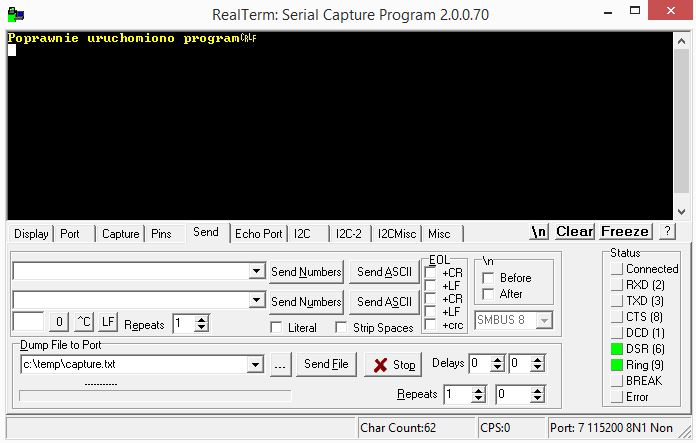
\includegraphics[width=4in]{realterm.jpg}
	\caption{Okno programu Realterm z komunikatem o poprawnym uruchomieniu programu.}
\end{figure}

\paragraph*{}
Rozmiar jednej komendy wysyłanej do układu Zynq wynosi 5 bajtów.
Pierwszy informuje o typie rozkazu, a 4 kolejne są danymi do tego rozkazu.
Każdy kolejny odebrany bajt umieszczany jest w buforze o rozmiarze 5 bajtów.
Włączone zostało przerwanie od pełnego bufora.
Po wysłaniu komendy z PC w procesorze układu Zynq uruchamiane jest przerwanie, w którym wysłany zostaje odpowiedni rozkaz do sterownika serwomechanizmów lub ustawiana jest zmienna informująca o pracy w trybie autonomicznym, podczas którego kamera ustawiana jest tak, by obiekt znajdował się w centrum kadru.
%TODO niejasne, bo wczesniej tryb autonomiczny sie nie pojawił. -zrobione.
Zaimplementowano obsługę następujących komend w Zynq:
\begin{itemize}
\item Zmiana pozycji serwomechanizmów: 0x00 0xHH 0xLL 0xHH 0xLL.
\item Zmiana maksymalnej prędkości serwomechanizmów: 0x01 0xHH 0xLL 0xHH 0xLL.
\item Zmiana maksymalnego momentu serwomechanizmów: 0x02 0xHH 0xLL 0xHH 0xLL.
\item Odczyt aktualnej wartości zadanej ze sterownika: 0x03 0x-- 0x-- 0x-- 0x--.
\item Rozpoczęcie pracy autonomicznej (śledzenia): 0x04 0x-- 0x-- 0x-- 0x--.
\end{itemize}
\paragraph*{}
W pierwszych trzech rozkazach pierwsze dwa bajty danych są parametrami dla serwomechanizmu odpowiedzialnego za obrót, a kolejne dwa są parametrami dla serwomechanizmu odpowiedzialnego za nachylenie. 
Myślniki w kolejnych komendach oznaczają, że wysłane bajty danych nie są istotne (komendy te nie potrzebują danych).

\section{Zynq-Maestro}
\label{sec:zynq-maestro}

% Tutaj wstaw zdjęcie połączonego układu ZYBO-Maestro.

Komunikacja przez UART została narzucona, gdyż jest to jedyny protokół komunikacyjny w Maestro. 
Połączone zostały odpowiednie piny (MIO 14,15) złącza MIO PMOD karty ZYBO do pinów Maestro odpowiadających za komunikację szeregową.
Następnie do użytych pinów MIO podłączono wyjścia innego układu procesora odpowiadającego za komunikację szeregową - UART0.
W dokumentacji Maestro wyszukano listę komend i zaimplementowano wysyłanie potrzebnych w układzie Zynq \cite{MM}. Są to następujące komendy:
\begin{itemize}
\item Zmiana pozycji serwomechanizmów: 0x9F 0x02 0x0A 0xLL 0xHH 0xLL 0xHH.
\item Zmiana maksymalnej prędkości serwomechanizmów: 0x87 0x0A/0x0B 0xLL 0xHH.
\item Zmiana maksymalnego momentu serwomechanizmów: 0x89 0x0A/0x0B 0xLL 0xHH.
\item Odczyt pozycji ze sterownika: 0x90 0x0A/0x0B.
\end{itemize}
W powyższych komendach A oznacza obrót, a B nachylenie (są to numery kanałów sterownika zapisane szesnastkowo).

\section{Testy komunikacji}
\label{testy_komunikacji}
Komunikacja była testowana na układzie złożonym z:
\begin{itemize}
\item Komputera klasy PC.
\item Karty ewaluacyjnej ZYBO.
\item Komputera Raspberry Pi 2 Model B.
\end{itemize}

\begin{figure}[h]
	\centering
	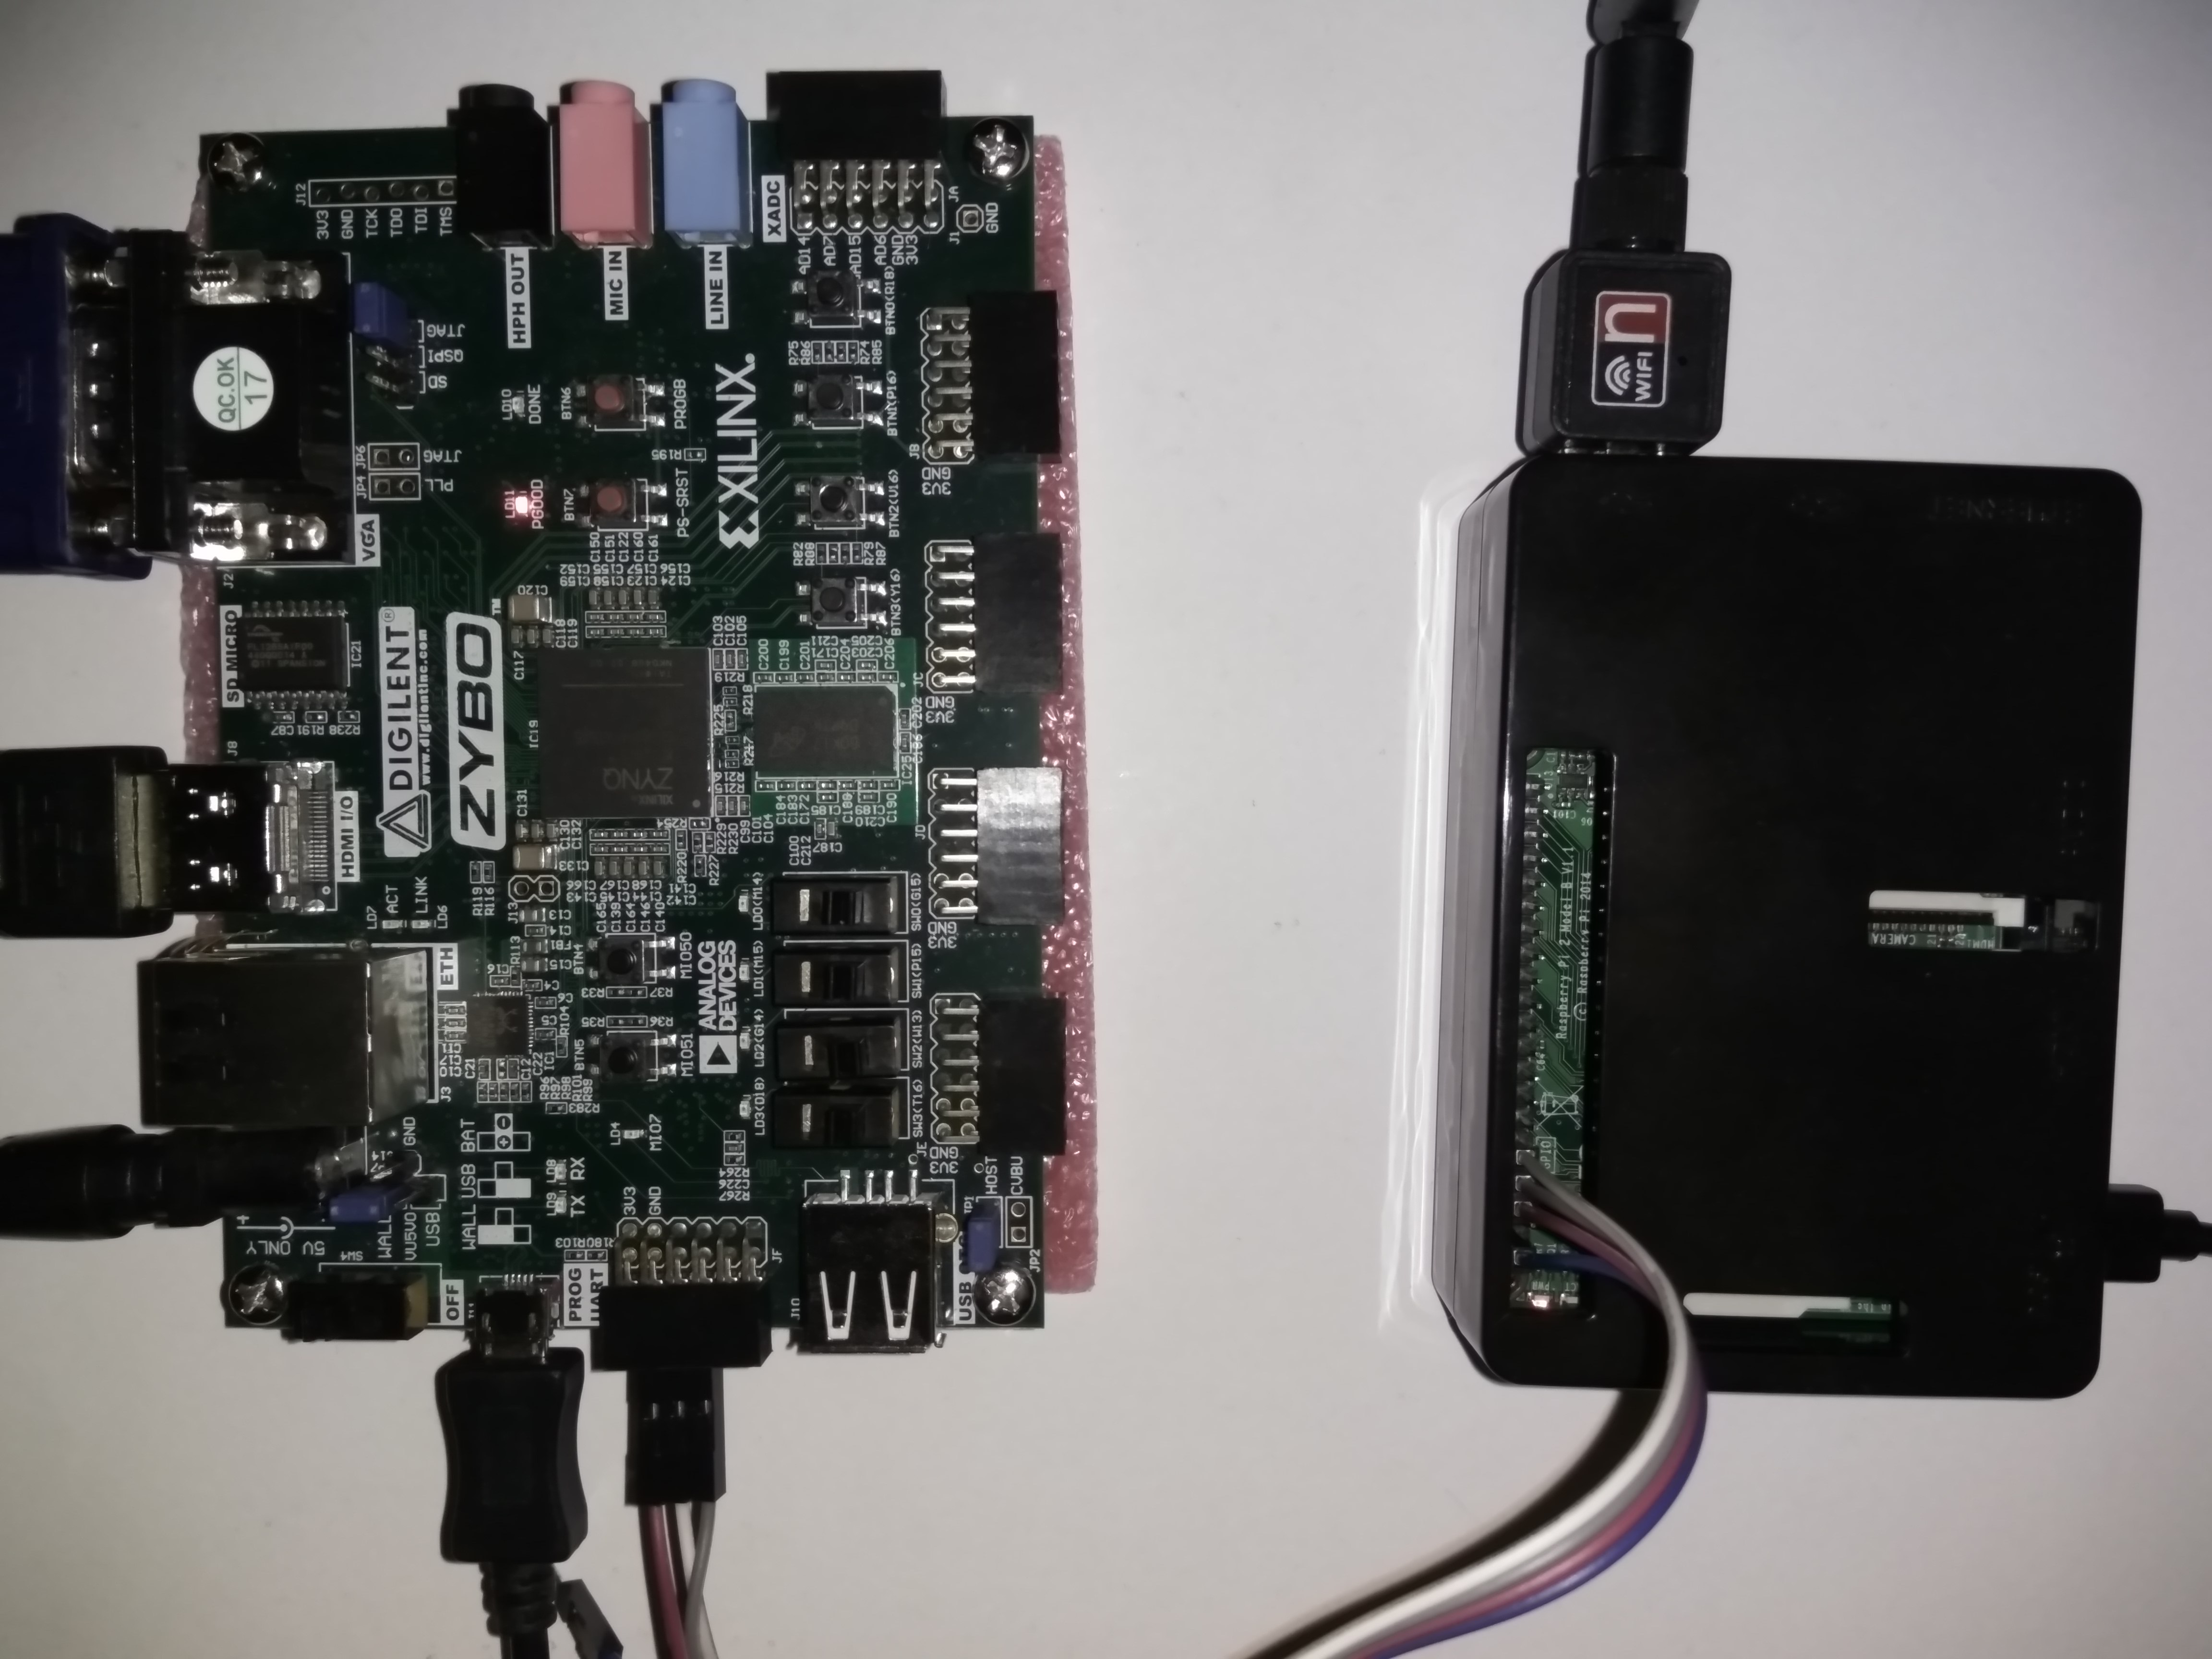
\includegraphics[width=4in]{raspberry.jpg}
	\caption{Karta ewaluacyjna ZYBO i komputer Raspberry pi 2 B użyty do testów.}
\end{figure}

\paragraph*{}
W układzie tym Raspberry zastępowało sterownik serwomechanizmów.
Zamiana ta została wykonana, by mieć możliwość sprawdzania poprawności danych odbieranych z Zynq.
W trakcie testów okazało się, że pierwszy bajt wysyłany do ZYBO jest wpisywany do bufora i wskaźnik jest przesuwany, lecz w kontrolerze przerwań nie jest zwiększany licznik liczby bajtów w buforze.
W efekcie przerwanie od pełnego bufora danych przychodzących było wywoływane o 1 bajt za późno (po otrzymaniu pierwszego bajtu nowej komendy).
Naprawiono to poprzez dodatkowy test w trakcie inicjalizacji komunikacji szeregowej.
Polegał on na włączeniu trybu \textit{loopback}, wysłaniu i odebraniu kilku bajtów danych, a następnie zresetowaniu bufora. W trybie \textit{loopback} dane wysyłane przez UART są wysyłane na jego wejście.
W ten sposób można sprawdzać zgodność danych.
Oprócz tego sprawdzono, czy wysłanie komendy z PC do Zynq skutkuje wysłaniem poprawnej komendy z Zynq do Maestro.
Po naprawieniu opisanego problemu i ponownym przeprowadzeniu testów stwierdzono, że komunikacja działa poprawnie.